%+++++++++++++++++++++++++++++++++++++++++++++++++++++++++++++++
% SUMMARY    : Lecture 15 
%            : Optimizers
%            : University of Southern Maine 
%            : @james.quinlan
%            : Gabrielle Akers - Lecture 15
%+++++++++++++++++++++++++++++++++++++++++++++++++++++++++++++++

\section*{Objectives}
\begin{outline}
    \1 Optimizers
    \1 Batch Gradient Descent
    \1 Momentum
    \1 RMSProp
\end{outline}

\rule[0.0051in]{\textwidth}{0.00025in}
% ----------------------------------------------------------------
\section{Optimizers}
\begin{enumerate}
    \item Batch Gradient Descent
    \newline In the past couple of classes we have been focusing primarily on Batch Gradient Descent and the math behind it.
    \newline \textbf{Issues}
    \begin{enumerate}
        \item Computationally expensive
        \newline Batch gradient descent computes the gradient at every single data point, which ensures points don't get passed over, but also requires a lot of needless computations
        \item Notational issues
        \[
        loss = l(w,x)
        \]
        \[
        L(w,x) = \frac{1}{n} \sum l(w,x)
        \]
        \[
        \nabla_w L(w,x)=\nabla (\frac{1}{n} \sum l(w,x)) = \frac{1}{n} \sum \nabla l(w,x)
        \]
        The derivative of a sum should be equal to the sum of the derivatives
        \item Slow convergence
        \newline The steps get progressively smaller
        \item Gets stuck on local minimums
    \end{enumerate}
    \textbf{Related Types of Gradient Descent}
    \begin{enumerate}
        \item Stochastic Gradient Descent (SGD)
        \newline This type of gradient descent selects a random x every time
        \[
        l(w,x_r)
        \]
        \item Minibatch Gradient Descent
        \newline A combination of SGD and Batch Gradient Descent. It uses a sample of x values and selects a random value from that sample for computation.
        \newline The general rule for the batch size is 32 or less.
        \[
        batchsize \leq 32
        \]
    \end{enumerate}
    \item Momentum
    \newline A type of gradient descent that takes into consideration previous gradients in order to prevent getting stuck at local minimums.
    \[
    w_{t+1}=w_t-\alpha \nabla_w L(w_t)-previous\ gradients
    \]
    \newline \textbf{Features}
    \begin{enumerate}
        \item Faster convergence than Batch Gradient Descent
        \item Doesn't get stuck at local minimums
        \item The amount of past gradients used are controlled with exponentially decaying weighted averages
        \[
        v_{t+1}=\beta v_t + (1-\beta)\nabla_wL(w_t)
        \]
        \[
        w_{t+1}=w_t-\alpha v_{t+1}
        \]
        Hyperparameters
        \[
        \alpha = learning\ rate
        \]
        \[
        \beta = weights
        \]
        \item Hyperparameters are tuned with cross validation
        \begin{align}
        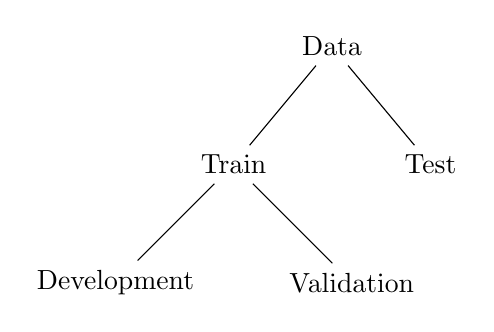
\begin{tikzpicture}
        [
        level 1/.style={sibling distance=25mm},
        level 2/.style={sibling distance=30mm},
        ]
	    \node {Data}
		child {node {Train}
                child {node {Development}}
                child {node {Validation}}
        }
		child {
		    node {Test}
		};
        \end{tikzpicture}
        \end{align}
        \newline The best practice has $\beta =0.9$, but it just has to be less than 1
        \item Update function
        \[
        w_{t+1} = \sum_{i=0}^{t} \beta^i(1-\beta)\nabla L_{t-i}
        \]
    \end{enumerate}
    \textbf{Issues}
    \begin{enumerate}
        \item Can overshoot and miss the global minimum
        \item Still can get stuck at some local minimums
    \end{enumerate}
    Unrolling the recurrence relation
    \[
    v_{t+1} = \beta v_t+(1-\beta)\nabla L_t
    \]
    \[
    v_{t+1} = \beta (\beta v_{t-1} +(1-\beta)\nabla L_{t-1})+(1-\beta)\nabla L_t
    \]
    \[
    v_{t+1}=\beta^2v_{t-1}+\beta(1-\beta)\nabla L_{t-1} +(1-\beta)\nabla L_t
    \]
    \[
    v_{t+1}=\beta^2(\beta v_{t-2}+(1-\beta)\nabla L_{t-2})+\beta(1-\beta)\nabla L_{t-1}+(1-\beta)\nabla L_t
    \]
    \[
    v_{t+1}=\beta^3v_{t-2}+\beta^2(1-\beta)\nabla L_{t-2}+\beta(1-\beta)\nabla L_{t-1}+(1-\beta)\nabla L_t
    \]
    \item RMSProp
    \newline A type of gradient descent that is adaptable depending on the size of the gradient
    \begin{align*}
    \nabla L(w) &= \begin{bmatrix}
           \delta L/\delta w_1    \\
           \delta L\delta w_2    \\
           \vdots   \\
           \delta L/\delta w_n    \\
         \end{bmatrix} \\
    \end{align*}
    \newline \textbf{Features}
    \begin{enumerate}
        \item Weighs gradients differently in different directions
        \begin{enumerate}
            \item Large gradient $\rightarrow$ Small step
            \item Small gradient $\rightarrow$ Large step
        \end{enumerate}
        \item Learning rates are different for each component
        \item Element wise operations
        \[
        \hspace{1.1cm} \rightarrow cross product \rightarrow vector
        \]
        \[
        uxv \rightarrow dot product \rightarrow scalar
        \]
        \[
        \hspace{2.3cm} \rightarrow Hadamard\ product \rightarrow vector
        \]
    \end{enumerate}
    \item AdaGrad
    \item NAG (Nestrov Accelerated Gradient)
    \item Adam
    \newline Created in 2015, Adam is generally considered to be the best type of gradient descent. It takes the best features of both Momentum and RMSProp and combines them into a single type of gradient descent.
\end{enumerate}
